\section{Вычисление факториала}
\subsection{Условие задания}
Разработать приложение для вычисления факториала по приведённому примеру.

Приложение должно содержать следующие компоненты:

\begin{enumerate}
  \item Заголовок формы должен отражать суть задания.
  \item Все элементы формы должны быть внятно подписаны (кнопки подписаны, у текстового поля должно быть написано, для чего оно нужно и т.д.)
  \item В коде должны быть комментарии и отступы (код должен быть легко читаем).
  \item В коде программы все элементы формы должны быть переименованы (btnName -  для кнопок, lblName - для ссылок, txtName - для текстового поля и т. д.) Наименования должны быть понятными.
  \item Приложение должно корректно работать (выводить ответ или ошибку с соответствующим сообщением) для следующих данных: ввод буквы, ввод отрицательного числа, ввод нуля, ввод положительного числа (< 10), ввод большого положительного числа. После вывода ошибок при вводе корректных данных поля ошибок должны очищаться.
\end{enumerate}

\subsection{Факториал натурального числа}
Факториалом натурального числа $n$ называют число $n!$, такое, что:

\begin{equation}
  n! = 1 \times 2 \times \dots \times (n - 1) \times n
\end{equation}

\subsection{Нахождение факториала рекурсивным способом}
В соответствии с алгоритмом вычисления факториала \cite{factorial-calculation},

$\forall n \in \mathbb{N} \text{ выполняется}$
\begin{itemize}
  \item $0 \leqslant n \leqslant 1 \Rightarrow n! = 1$;
  \item $n > 1 \Rightarrow n! = (n-1)!\times n$.
\end{itemize}
В силу ограниченного размера регистров процессора на $n$ накладывается ограничение $n \leq 22$.

\subsection{Вид формы в конструкторе}
Форма имеет вид:
\begin{figure}
  \centering
  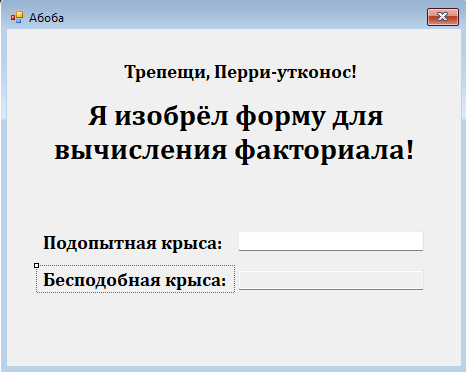
\includegraphics[width=0.5\linewidth]{images/factorial/form.png}
  \caption{Форма окна для вычисления факториала}
  \label{fig:factorial-form}
\end{figure}

\subsection{Таблица с описанием элементов формы}
Все элементы формы были переименованы. В таблице \ref{tab:factorial-form} представлены все изменения.

\begin{table}[H]
  \centering
  \begin{tabular}{|m{0.3\textwidth}|m{0.3\textwidth}|m{0.3\textwidth}|}
    \hline
    \textbf{Описание элементов формы} & \textbf{Список изменённых атрибутов} & \textbf{Новое значение атрибута} \\
    \hline
    \hline
    Окно формы & Text & Абоба \\
    Верхний подзаголовок & Name & lblSubtitle \\
    Верхний заголовок & Name & lblTitleStart \\
    Нижний заголовок & Name & lblTitleEnd \\
    Метка поля ввода & Name & lblInput \\
    Метка поля вывода & Name & lblOutput \\
    Поле ввода & Name & textInput \\
    Поле вывода & Name & textOutput \\
    \hline
  \end{tabular}
  \caption{Значение атрибутов элементов в приложении для вычисления факториала}
  \label{tab:factorial-form}
\end{table}

\subsection{Примеры правильной и неправильной работы приложения}
При запуске приложения на экране появляется окно \ref{fig:factorial-start}.
\begin{figure}
  \centering
  
\includegraphics[width=0.5\linewidth]{images/factorial/start.png}
  \caption{Запуск программы}
  \label{fig:factorial-start}
\end{figure}

При вводе реактивно подсчитывается и подставляется значение в поле вывода. Также реактивно происходит обработка ошибок.

\begin{figure}
  \centering
  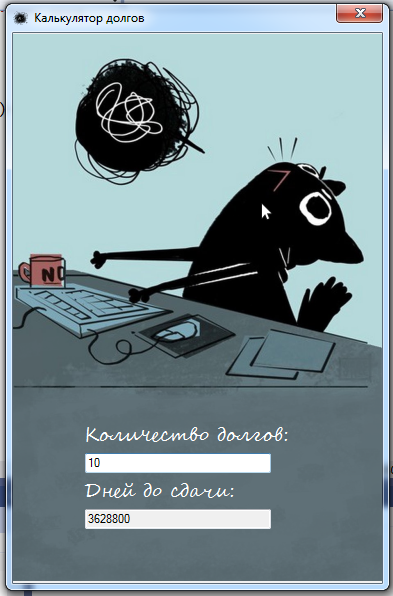
\includegraphics[width=0.5\linewidth]{images/factorial/okay.png}
  \caption{Запуск программы с корректными данными}
  \label{fig:factorial-okay}
\end{figure}

\begin{figure}
  \centering
  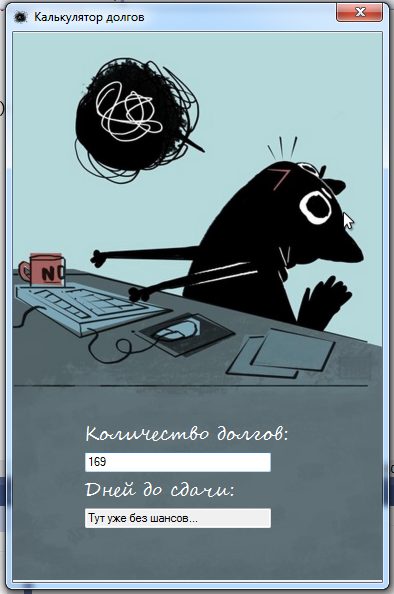
\includegraphics[width=0.5\linewidth]{images/factorial/error.png}
  \caption{Запуск программы с некорректными числовыми данными}
  \label{fig:factorial-error}
\end{figure}

\begin{figure}
  \centering
  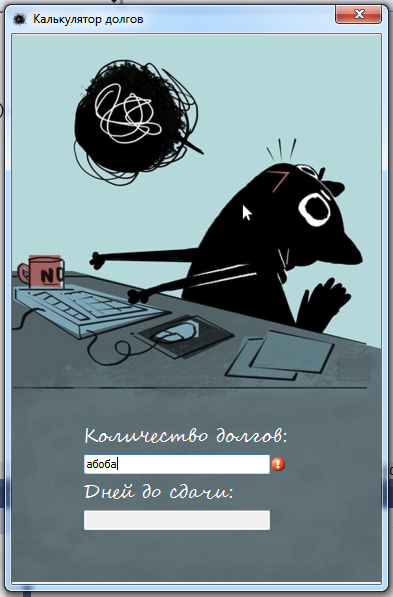
\includegraphics[width=0.5\linewidth]{images/factorial/error2.png}
  \caption{Запуск программы с нечисловыми данными}
  \label{fig:factorial-error2}
\end{figure}

\subsection{Примеры исходного кода}
\begin{minted}{cpp}
/// Функция вычисления факториала, принимает n в [0,FACTORIALIZER_MAX_N)
long long Factorializer::factorial(long long n) {
	if (n > FACTORIALIZER_MAX_N) {
		throw gcnew System::ArgumentOutOfRangeException("результат превысит 64 бит, операция не позволена");
	} else if (n < 0) {
		throw gcnew System::ArgumentOutOfRangeException("факториал отрицательного числа не определён");
	} else if (n == 0) {
		return 1;
	}
	if (!(*used)[n - 1]) {
		dp[n - 1] = n * factorial(n - 1);
		(*used)[n - 1] = true;
	}
	return dp[n - 1];
}

/// Конструктор вычислителя факториала
Factorializer::Factorializer() {
	dp = (long long*)calloc(FACTORIALIZER_MAX_N, sizeof(long long));
	used = new std::bitset<FACTORIALIZER_MAX_N>(0);
}

/// Конструктор копирования факториала
Factorializer::Factorializer(const Factorializer %) {
	dp = nullptr;
	used = new std::bitset<FACTORIALIZER_MAX_N>();
	throw gcnew System::InvalidOperationException("не надо пытаться копировать единое состояние, пожалуйста");
}
\end{minted}

Больше кода проекта доступно в приложении \ref{application-A}. Также в приложенном архиве можно найти полный код проекта.